\documentclass[border=12pt]{standalone}
\usepackage{tikz}
\usetikzlibrary{shapes,backgrounds,positioning}

\begin{document}
\sffamily
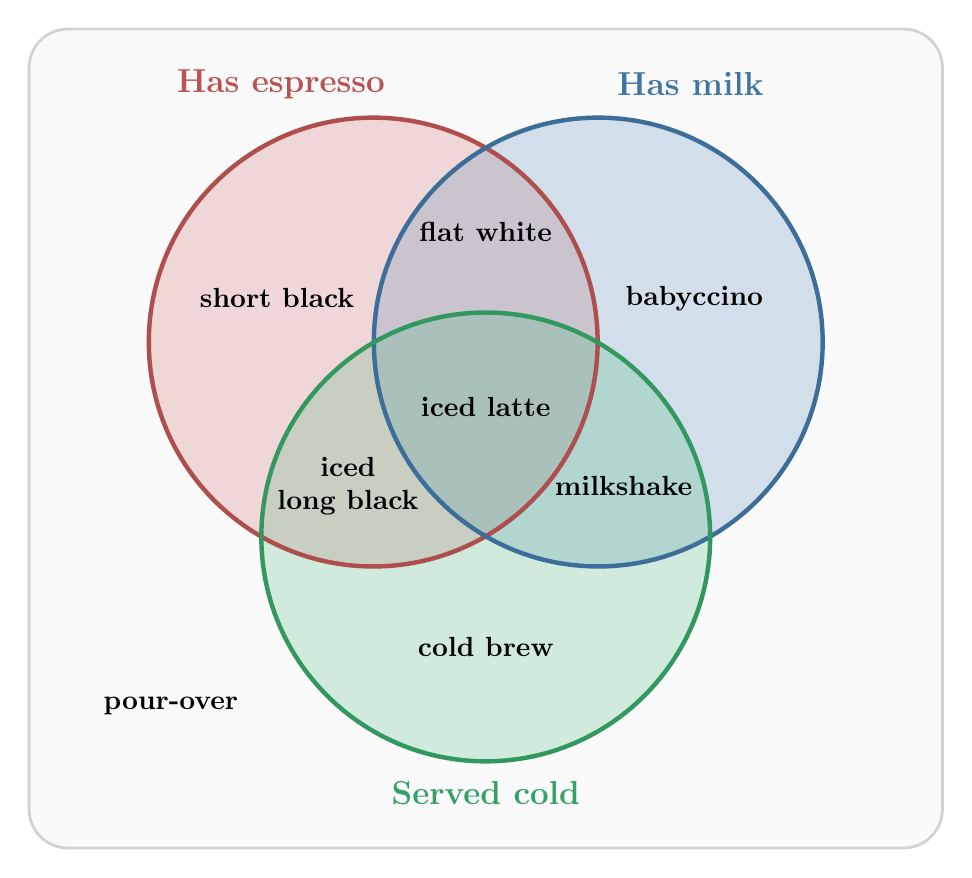
\begin{tikzpicture}[thick]
  % Define harmonious colors for the three sets
  \definecolor{cEspresso}{RGB}{205, 92, 92}   % Indian Red
  \definecolor{cMilk}{RGB}{70, 130, 180}       % Steel Blue
  \definecolor{cCold}{RGB}{60, 179, 113}       % Sea Green

  % Bounding box representing universal set of drinks
  \draw[rounded corners=14pt, fill=gray!4, draw=gray!35, line width=1pt] (-5.8, -5.6) rectangle (5.8, 4.8);

  % Circle coordinates: r0 = 1.65, R = 2.85
  % C1 (Espresso): 150 deg -> (-1.429, 0.825)
  % C2 (Milk):      30 deg -> ( 1.429, 0.825)
  % C3 (Cold):     270 deg -> ( 0.000, -1.650)

  % Circle fills with transparency
  \begin{scope}[fill opacity=0.22]
    \fill[cEspresso] (-1.429, 0.825) circle (2.85);
    \fill[cMilk]      (1.429, 0.825) circle (2.85);
    \fill[cCold]      (0.000, -1.650) circle (2.85);
  \end{scope}

  % Circle outlines
  \draw[cEspresso!85!black, line width=1.6pt] (-1.429, 0.825) circle (2.85);
  \draw[cMilk!85!black,     line width=1.6pt] ( 1.429, 0.825) circle (2.85);
  \draw[cCold!85!black,     line width=1.6pt] ( 0.000, -1.650) circle (2.85);

  % Circle Headings / Labels
  \node[cEspresso!90!black, font=\bfseries\large] at (-2.6, 4.1) {Has espresso};
  \node[cMilk!90!black,     font=\bfseries\large] at ( 2.6, 4.1) {Has milk};
  \node[cCold!90!black,     font=\bfseries\large] at ( 0.0, -4.9) {Served cold};

  % Drinks placement: exactly one per Venn diagram region
  % 1. Has espresso only
  \node[align=center, font=\bfseries] at (-2.65, 1.38) {short black};

  % 2. Has milk only
  \node[align=center, font=\bfseries] at (2.65, 1.38) {babyccino};

  % 3. Served cold only
  \node[align=center, font=\bfseries] at (0.00, -3.05) {cold brew};

  % 4. Has espresso + Has milk (not cold)
  \node[align=center, font=\bfseries] at (0.00, 2.22) {flat white};

  % 5. Has espresso + Served cold (no milk)
  \node[align=center, font=\bfseries] at (-1.75, -1.00) {iced\\long black};

  % 6. Has milk + Served cold (no espresso)
  \node[align=center, font=\bfseries] at (1.75, -1.00) {milkshake};

  % 7. Has espresso + Has milk + Served cold (center)
  \node[align=center, font=\bfseries] at (0.00, 0.00) {iced latte};

  % 8. Outside all three circles (Universal set)
  \node[align=center, font=\bfseries] at (-4.00, -3.80) {pour-over};

\end{tikzpicture}
\end{document}
